%%%%%%%%%%%%%%%%%%%%%%%%%%%%%%%%%%%%%%%%%%%%%%%%%%%%%%%%%
\section{Scenario}
\label{sec:scenario}

The tests take place in the \iterm{RoboCup@Home arena}. In addition, particular tests are situated outside the arena, e.g., in a previously unknown public place. The following rules are related to the \iterm{RoboCup@Home arena} and its contents. 

\subsection{RoboCup@Home arena}
The \iterm{RoboCup@Home arena} is a realistic home setting consisting of inter-connected rooms like, for instance, a living room, a kitchen, a bath room, and a bed room. 

% \subsection{Team area}\label{rule:scenario_team_area}

% \todo{remove? does not depend on the rules, but on local organization }
% The maximum number of people to register per team is unlimited, but
% the organization only provides space for \emph{four} (4) persons to
% work at tables in the team area. 
% \todo{this is actually more an additional note for the registration information}

\subsection{Walls, doors and floor}
\label{rule:scenario_walls}

The indoor home setting will be surrounded by high and low \Term{walls}{Arena walls}. These walls will be built up using standard fair construction material.

\begin{enumerate}
	{\bf\item Walls:} Walls have a minimum height of \SI{60}{\centi\meter}. A maximum height is not specified, but should be chosen so that the audience is able to watch the competition.\\
	Walls will be fixed and are likely to be not modified during the competition (see \refsec{rule:scenario_changes}). 

	{\bf\item Doors:} There will be at least two entry/exit \Term{doors}{Arena doors} connecting the outside of the scenario. These doors are used as starting points for the robots (see \refsec{rule:start_position}).
	% At least one of the entrances will be a door with a handle (not a knob).\
	There will be also another door inside the scenario with a handle (not a knob) between any two rooms.

	{\bf\item Floor:} The floor of the arena as well as the doorways of the arena are even. That is, there will be no significant steps or even stairways. However, minor unevenness such as carpets, transitions in floor covering between different areas, and minor gaps (especially at doorways) must be expected.

	{\bf\item Appearance:} Floor and walls are mainly uni-colored but can contain texture, e.g., a carpet on the floor, or a poster or picture on the wall.\\
	Although being unlikely at the moment, transparent elements are also possible. 
\end{enumerate}


\subsection{Furniture}
\label{rule:scenario_furniture}

The arena will be equipped with typical objects (furniture) that are not specified in quantity and kind. The minimal configuration consists of 
\begin{itemize}
	\item a small dinner table with two chairs, 
	\item a couch, 
	\item an open cupboard or small table with a television and remote control, 
	\item a cupboard or shelf (with some books inside), and
	\item a refrigerator in the kitchen (with some cans and plastic bottles inside). 
\end{itemize}
A typical arena setup is shown in \reffig{fig:scenario_arena}.

\begin{figure}[tbp]
	\centering
	\subfloat[Typical arena]{\label{fig:scenario_arena}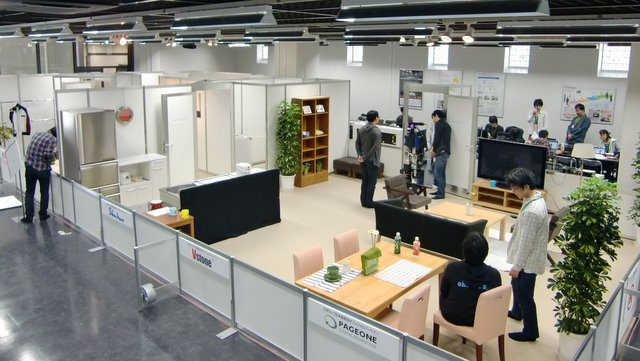
\includegraphics[height=46mm]{images/typical_arena.jpg}} ~ 
	\subfloat[Typical objects]{\label{fig:scenario_objects}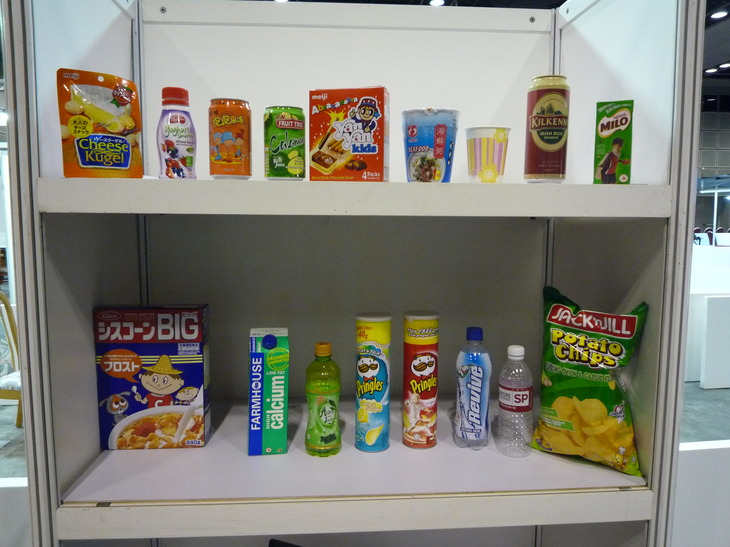
\includegraphics[height=46mm]{images/typical_objects.jpg}}
	\caption{Scenario examples: (a) a typical arena, and (b) typical objects.}
	\label{fig:arena}
\end{figure}



\subsection{Changes to the arena}
\label{rule:scenario_changes}

Since the robots should be able to function in the real world the scenario is not fixed and might change without further notice.
\begin{enumerate}
	{\bf\item Major changes:} Changes will primarily influence the position of objects such as furniture inside the arena while walls are likely to stay fixed. Multiple changes may take place up to completely restructuring the internals of the apartment. The position of named locations (see \refsec{rule:scenario_names}) are not changed when used in a test, e.g., as navigation goal. \\
	In addition, passages may be blocked and cleared, respectively. One hour before a test slot begins no \iterm{major changes} will be made.

	{\bf\item Minor changes:} In contrast to major changes, \iterm{minor changes} like, for instance, slightly moved chairs cannot be avoided and may happen at any time (even during a test). 
\end{enumerate}


\subsection{Predefined objects}
\label{rule:scenario_objects}

\def\NumObjects{25\ }
\def\NumLocations{20\ }
\def\NumNames{20\ }

Some tests in the RoboCup@Home league involve the manipulation of objects. These objects resemble items usually found in household environments like, for instances, soda cans, coffee mugs or books. An example of objects used in a previous competition can be seen in \reffig{fig:scenario_objects}.

\begin{enumerate}
	{\bf\item Definition:} The TC will compile a list of \NumObjects objects. There are no restrictions on object size, appearance or weight. % (YES, this sentence is NOT NEW, but have been in the old rulebook!) 
	However, it can be expected that the selected objects are easily manipulable by a human using a single hand.
	{\bf\item Object classes:} Each object will be assigned to an \iterm{object class}. The objects \quotes{lemonade} and \quotes{ice tea} may be of class \quotes{beverage} for example.

	{\bf\item Object (class) locations:} Each object (class) will be assigned to an \iterm{object location}. Objects of class \quotes{drink} may be usually found on the \quotes{kitchen table} for example.

	{\bf\item Announcement:} The TC makes the set of objects (and their names, classes, and usual locations) available during the setup days.

	{\bf\item Known vs.\ unknown}: These objects are used as the \iterm{known objects} in the test specifications; \iterm{unknown objects} are not taken from the set of \iterm{predefined objects}. 
	
	{\bf\item Placement:}\nterm{object placement} In manipulation tasks, the objects will be positioned at \iterm{manipulation locations} and less than \SI{15}{\centi\meter} away from the border of the surface they are located at. There will be at least 5cm space around each object.
\end{enumerate}



\subsection{Predefined locations}
\label{rule:scenario_locations}

Some tests in the RoboCup@Home league involve \iterm{predefined locations}. 
These may include places like a \quotes{bookshelf} or a \quotes{dining table}, as well as certain objects such as a \quotes{television}, or the \quotes{front door}. 

\begin{enumerate}
	{\bf\item Definition:} The TC will compile a list of predefined locations. There are no restrictions on which parts of the arena will be selected as a predefined location.

	{\bf\item Location classes:} Each location will be assigned to a \iterm{location class}. The objects \quotes{couch} and \quotes{arm chair} may be of class \quotes{seat} for example. 

	{\bf\item Announcement:} The TC makes the set of locations (and their names and classes) available during the setup days.

	{\bf\item Position:} The positions of locations are \emph{not} necessarily fixed (see \refsec{rule:scenario_changes}).

	{\bf\item Manipulation locations:} The TC will mark \NumLocations locations out of the set of predefined locations as being \iterm{manipulation locations}. Whenever a test involves manipulation, the object to manipulate will be placed at one of the manipulation locations. 
\end{enumerate}



\subsection{Predefined rooms}
\label{rule:scenario_rooms}
Some tests in the RoboCup@Home league involve \iterm{predefined rooms}. 
\begin{enumerate}
	{\bf\item Definition:} The TC will compile a list of room names.
	{\bf\item Announcement:} The TC makes the set of rooms available during the setup days.
\end{enumerate}



\subsection{Predefined (person) names}\label{rule:scenario_names}

Some tests in the RoboCup@Home league involve \iterm{predefined names} of people. 

\begin{enumerate}
	{\bf\item Definition:} The TC will compile a list of \NumNames predefined names. The names are \SI{50}{\percent} male and \SI{50}{\percent} female, and taken from the (current) most common first names in the United States.\\
	In order to ease speech recognition, it is tried to select names to be phonetically different from each other.

	{\bf\item Announcement:} The TC makes the set of names available during the setup days.
	{\bf\item Assignment:} When a test involves interacting with persons (using a person's name), all involved persons are assigned names by the referees before the test. 
\end{enumerate}

Typical names are, for example, James, John, Robert, Michael and William as male names; Mary, Patricia, Linda, Barbara and Elizabeth as female names.


%% %%%%%%%%%%%%%%%%%%%%%%%%
\subsection{Wireless network}\label{rule:scenario_wifi}

For wireless communication, an \iterm{arena network} is provided. The actual infrastructure depends on the local organization. 

\begin{itemize}
	\item To avoid interference with other leagues, this WiFi has to be used for communication only. It is not allowed to use the above or any other WiFi network for personal use at the venue.
	\item During the competitions, only the active team is allowed to use the \iterm{arena network}. 
	\item The organizers cannot guarantee reliability and performance of wireless communication. Therefore, teams are required to be ready to setup, start their robots and run the tests even if, for any reason, network is not working properly.
\end{itemize}

Preferably the organizers will try to provide one LAN cable on the desk of each participating team for Internet connection. However, this cannot be guaranteed. If multiple LAN connections are needed, each team has to bring its own LAN hub/switch and cables.

\paragraph*{Important note:} Any unapproved wireless device may be removed by the TC at any time.

\subsection{Smart Home Devices}\label{rule:smarthomedevices}

\todo{Finish writing this section.}
There is a list of official devices that can be used in some tests for additional score. The protocol to communicate with these devices will be provided well beforehand the competition.

